\documentclass[11pt,a4paper]{article}

\usepackage{polski}
%kodowanie widnows
%\usepackage[cp1250]{inputenc} 
%kodowanie linux
\usepackage[utf8]{inputenc}


%\usepackage[T1]{fontenc}
\usepackage{indentfirst}
\usepackage{wrapfig}    % for wrapping figures, tables

\frenchspacing

\usepackage{amssymb}
%\usepackage{bm}
\usepackage{gensymb}
%\usepackage{hepnames}
\usepackage{epsfig}
\usepackage{graphics}
\usepackage[shortlabels]{enumitem}
%\usepackage{xspace}
%\xspaceaddexceptions{[]\{\}}

%
%
%fixpagesize
\pagestyle{empty}
\addtolength{\textwidth}{6cm}
\addtolength{\textheight}{4cm}
\addtolength{\evensidemargin}{-3cm}
\addtolength{\oddsidemargin}{-3cm}
\addtolength{\topmargin}{-2cm}
\parindent=0cm


%
%
%small distance in list/item/enum for enumitem package
\setlist[itemize,enumerate]{topsep=0em}
\setlist{noitemsep}

%print zadanie #
\newcounter{zadanie}\newcommand{\zadanie}[1][]{\addtocounter{zadanie}{1} ~\\  {\bf \emph{Zadanie \arabic{zadanie} #1 }} \\}
\newcounter{zaddom}\newcommand{\zaddom}[1][]{\addtocounter{zaddom}{1} ~\\  {\bf \emph{Zadanie domowe \arabic{zaddom} #1 }} \\}
%\renewcommand{\zadanie}[1][]{\pagebreak  ~\\  {\bf \emph{Zadanie }} \\} \addtolength{\topmargin}{-2cm}


%%%%%%%%%%%%%%%%%%%%%%%%%%%%%%%%%%%%%%%%%%%%%%%%%%%%%%
\begin{document}           % End of preamble and beginning of text.
\vspace*{-1.8cm}

\begin{centering}
\bf{\Large{Termodynamika z elementami fizyki statystycznej}}\\
Ćwiczenia 3 \\[1mm]
ciśnienie, pływanie, równanie stanu, gaz doskonały \\
\end{centering}

\zadanie
Zależność objętości od ciśnienia dla pewnej substancji dana jest empirycznym wzorem $V(p) = V_0(1 + a\cdot p)^{-\alpha}$.
Wykazać, że w takim przypadku współczynnik ściśliwości $\kappa=-1/V(\partial V(p,T)/\partial p)_T$ spełnia relację: $1/\kappa=1/\kappa_0+c\cdot p$.
Wyznaczyć stałe $\kappa_0$ i $c$ przez $a$ i $\alpha$.

\vspace{2mm}{\bf Rozwiązanie}: Podstawiając do wzoru znajdujemy
\[
\kappa(p)=\frac{\alpha\,a}{1+a\,p}
\]
zatem
\[
\frac{1}{\kappa(p)}=\frac{1}{\alpha\,a}+\frac{1}{\alpha}p=\frac{1}{\kappa_0}+c\,p
\]
gdzie $\kappa_0=\alpha\,a$, $c=1/\alpha$.

\clearpage

\zadanie
Okręt podwodny o stalowym kadłubie i masie m = $1000\textrm{t}$ jest zanurzony na głębokości peryskopowej tak, że siła wyporu jest dokładnie równa ciężarowi okrętu (pływalność zerowa). Temperatura wody wynosi przy tym 10\degree C. O ile trzeba zmienić balast okrętu, żeby utrzymać zerową pływalność po wpłynięciu na wodę o temperaturze 20\degree C? Współczynnik rozszerzalności objętościowej wody w tym zakresie temperatur wynosi $\gamma_w = 1.5\,10^{-4} K^{-1}$, zaś współczynnik rozszerzalności liniowej stali $\alpha_s = 1.2\,10^{-5} K^{-1}$. Ściśliwość wody i stali można zaniedbać.

\vspace{2mm}{\bf Rozwiązanie}:

Na okręt działają dwie przeciwnie skierowane siły, siła wyporu $F_w$ i siła ciężkości $F_g$
$F_w = \rho_w g V$, $F_g = mg$. (3) Pływalność zerowa oznacza równowagę tych dwóch sił: $F_w = F_g$ co pozwala nam wyznaczyć objętość okrętu:
\[
V = \frac{m}{\rho_w}
\]
Po wpłynięciu na cieplejsze wody zmieni się gęstość wody jak i objętość okrętu. Nowa gęstość wody wyniesie:
\[
\rho'_w = \rho_w \frac{1}{1+\gamma_w\,\Delta T}
\]
Nowa objętość okrętu to
\[
V' = V (1+3\alpha_s \Delta T)
\]
co prowadzi do nowego warunku pływalności:
\[
V' = \frac{m'}{\rho_w'}
\]
i w wyniku daje:
\[
m' = V'\,\rho'_w = m \frac{1+3\alpha_s \Delta T}{1+\gamma_w\,\Delta T} = m\,\big(1+(3\alpha_s-\gamma_w) \Delta T\big)
\]
Po podstawieniu danych:
\[
m'-m=m (3\alpha_s-\gamma_w) \Delta T = -0.0011\,\textrm{ton}
\]
czyli okręt musi zmniejszyć balast o jedną tone.

\clearpage

\begin{minipage}{0.75\textwidth}
\zadanie
Kulka znajduje się w stanie równowagi pomiędzy dwoma cieczami (rysunek A) o~gęstościach $\rho_1 = 1.0\textrm{g}/\textrm{cm}^3$ i~$\rho_2 = 0.8\textrm{g}/\textrm{cm}^3$. Objętość zanurzona w cieczy ``1'' jest dwa razy większa niż objętość zanurzona w cieczy ``2''. Oblicz gęstość kulki.\\\\\\\\\\\\\\\\\\
\end{minipage}
\begin{minipage}{0.25\textwidth}
\begin{center}

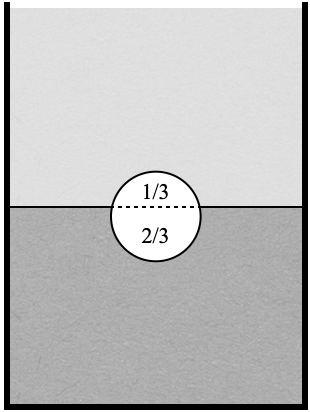
\includegraphics[width=0.8\textwidth]{zadanie3.png}
\end{center}
\end{minipage}

\vspace{2mm}{\bf Rozwiązanie}:\\
Skoro kulka jest w stanie równowagi pomiędzy dwoma cieczami to odpowiednie siły wyporu muszą bilansować siłę ciężkości:
\[
\rho_1\,V_1\,g + \rho_2\,V_2\,g = \rho_k (V_1 + V_2) g
\]
Wiedząc, że $V_1 = 2 V_2$ dostajemy
\[
\rho_k = \frac{\rho_1 V_1 +\rho_2 V_2}{V_1 + V_2} = \frac{1}{3}(2\rho_1 +\rho_2)
\]
Podstawiając dane: $\rho_k = 0.93\,\textrm{g/cm}^3$.

\clearpage

\zadanie
Ile moli i ile cząsteczek powietrza znajduje się w sali ćwiczeniowej?

\vspace{2mm}{\bf Rozwiązanie}:
Przyjmujemy, że powietrze jest gazem doskonałym. Przyjmijmy, że w sali panuje ciśnienie $p = 1000\,\textrm{hPa}$ i temperatura $T = 300\,\textrm{K}$. Przyjmijmy, że objętość sali to V = $3\times 5\times 10\,\textrm{m}^3$.
Z równania stanu gazu doskonałego dostajemy:
\[
n = \frac{p\,V}{R\,T} \approx 6000\,\textrm{mol}
\]
gdzie skorzystaliśmy, że stała gazowa $R \approx 8.31 \textrm{J}/(\textrm{mol}\,\textrm{K})$.\\
Liczbę cząsteczek $N$ można oszacować jako $N = n\,N_A \approx 3.6\,10^{27}\,\textrm{czasteczek}$.

\clearpage

\zadanie
Dla gazu doskonałego znajdź współczynniki:
\begin{itemize}
\item[1.] rozszerzalności objętościowej,
\item[2.] ściśliwości izotermicznej,
\item[3.] temperaturowej zmiany ciśnienia.
\end{itemize}

\vspace{2mm}{\bf Rozwiązanie}:\\
Korzystamy z równania stanu gazu doskonałego: $p\,V = n\,RT$:

\begin{itemize}
\item[1.] rozszerzalność objętościowa:
 \[
  \gamma = \frac{1}{V}\bigg(\frac{\partial V}{\partial T}\bigg)_p = 
  \frac{1}{V}\bigg(\frac{\partial}{\partial T}\frac{n\,RT}{p}\bigg)_p = \frac{n\,R}{p\,V}=\frac{1}{T}
 \]
\item[2.] ściśliwość izotermiczne:
 \[
  \kappa = -\frac{1}{V}\bigg(\frac{\partial V}{\partial p}\bigg)_T =
  -\frac{1}{V}\bigg(\frac{\partial}{\partial p}\frac{n\,RT}{p}\bigg)_T = \frac{n\,RT}{p^2\,V} = \frac{1}{p}
 \]
\item[3.] temperaturowej zmiana ciśnienia przy stałej objętości,
 \[
  \beta = \frac{1}{p}\bigg(\frac{\partial p}{\partial T}\bigg)_V =
  \frac{1}{p}\bigg(\frac{\partial}{\partial T}\frac{n\,RT}{V}\bigg)_V = \frac{n\,R}{p\,V} = \frac{1}{T}
 \]
\end{itemize}


\clearpage

\zadanie
W pionowym, znajdującym się w polu grawitacyjnym, zamkniętym cylindrze znajduje się gaz doskonały oraz dzielący naczynie masywny tłok, który może przemieszczać się bez tarcia. Z obu stron tłoka znajdują się jednakowe liczby cząstek gazu doskonałego. W temperaturze $T_0$, jednakowej w całym cylindrze, objętość górnej części jest $m$ razy większa niż objętość części dolnej. Jaki będzie stosunek tych objętości, jeśli temperatura wzrośnie do wartości $T_1$? Zaniedbać zmienność ciśnienia gazu z wysokością (tj. założyć, że w każdej z części cylindra ciśnienie jest stałe).

\vspace{2mm}{\bf Rozwiązanie}: Warunek równowagi sił $F_1 + M\,g = F_2$, gdzie $F_1$ ($F_2$) jest siłą wywieraną na tłok przez gaz znajdujący się w górnym (dolnym) zbiorniku a M jest masą tłoka. Oznaczając przez $S$ pole powierzchni tłoka dostajemy:
\[
p_1 + \frac{M\,g}{S} = p_2
\]
Powiążemy teraz $p_1$ i $p_2$ ze sobą korzystając z równania stanu gazu doskonałego.
Wiem, że $V_1 = n\,V_2$ gdzie $V = V_1 + V_2$. Z równania stanu gazu dla dolnego i górnego zbiornika w tej samej temperaturze dostajemy:
\[
1=\frac{p_1\,V_1}{p_2\,V_2} = m\frac{p_1}{p_2} \qquad\Rightarrow\qquad p_2=m\,p_1
\]
czyli warunek równowagi przybiera postać
\[
p_1 (m-1) = \frac{M\,g}{S}
\]
Na koniec, ponownie korzystając z równania Clapeyrona, możemy powiązać $p_1$ z temperaturą $T_0$ i stosunkiem objętości $n$ dostajemy:
\[
p_1 = \frac{NkT_0}{V_1} = \frac{m+1}{m}\frac{n\,RT_0}{V}
\]
Ostatecznie, warunek równowagi przybiera postać:
\[
\frac{m^2-1}{m}\frac{n\,RT_0}{V} = \frac{Mg}{S}
\]
Jeżeli temperatura wzrośnie do $T_1$ to warunek równowagi przybierze postać
\[
\frac{m'^2-1}{m}\frac{n\,RT_1}{V} = \frac{Mg}{S}
\]
        
gdzie $m'$ jest szukanym stosunkiem objętości. Porównując oba warunki równowagi dostajemy
\[
\frac{m'^2-1}{m}\frac{n RT_1}{V}=\frac{m^2-1}{m}\frac{n RT_0}{V}
\qquad\to\qquad
\frac{m'^2-1}{m}=\frac{m^2-1}{m}\frac{T_0}{T_1}\equiv \alpha
\]
Otrzymujemy równanie kwadratowe na $n'$:
\[
m'^2 - \alpha m' - 1 = 0
\]
którego rozwiązaniem z $n' > 0$ jest:
\[
m' = (\alpha + \sqrt{\alpha^2 + 4})/2\,\quad\textrm{gdzie:}\qquad \alpha = \frac{m^2-1}{m}\frac{T_0}{T_1}
\]

\clearpage

\zadanie
Wykazać, że dla gazu doskonałego zachodzi: $p = p_0 (1 + \frac{1}{273.15} T[\degree \textrm{C}])$ przy $V = \textrm{const}$,
oraz $V = V_0 (1+ \frac{1}{273.15}  T[\degree \textrm{C}])$ przy $p=\textrm{const}$, gdzie $p_0 =p(0\degree \textrm{C})$ i $V_0 =V(0\degree \textrm{C})$.

\vspace{2mm}{\bf Rozwiązanie}:\\
Korzystamy z równania stanu gazu doskonałego, przy stałej objętości (i liczbie moli gazu) znajdujemy związek:
\[
\frac{p}{T} = \frac{p_0}{T_0}
\]
Wyznaczając z niego $p$ i zapisując $T[\degree C] = (T - T_0)/(1\,\textrm{K})$, gdzie $T_0 = 273.15\,\textrm{K}$ otrzymujemy:
\[
p=p_0 \bigg(1+\frac{1}{273.15}T[\degree C]\bigg) .
\]
Postępując podobnie, przy założeniu, że tym razem ciśnienie jest stałe, znajdujemy drugi związek.

\clearpage

\begin{minipage}{0.75\textwidth}
\zadanie
„Nurek” szklany ma kształt walca zamkniętego od góry i otwartego od dołu i pływa po powierzchni wody, nad którą panuje ciśnienie $p_0 = 1\,\textrm{bar}$ w taki sposób, że $h_1 = 2\textrm{mm}$ wystaje nad powierzchnię. Wewnątrz nurka jest powietrze, którego słupek ma wysokość $h_2 = 2\,\textrm{cm}$.
Jakie powinno być ciśnienie $p_0$ nad powierzchnią wody, aby nurek zatonął? Powietrze traktujemy jako gaz doskonały, jego masę zaniedbujemy. Grubość ścianek naczynia zaniedbujemy. Temperatura wody jest taka sama jak temperatura otoczenia.\\\\\\\\

\end{minipage}
\begin{minipage}{0.25\textwidth}
\begin{center}

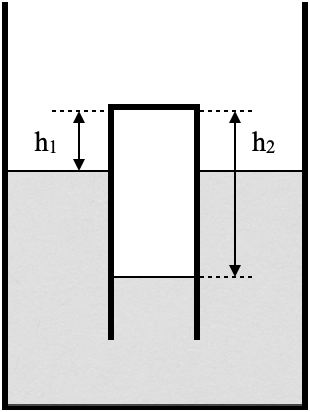
\includegraphics[width=0.8\textwidth]{zadanie8.png}
\end{center}
\end{minipage}

\vspace{2mm}{\bf Rozwiązanie}:\\
Niech $S$ będzie przekrojem nurka a m jego masą. Możemy napisać dwa równania. Pierwsze jest warunkiem pływania nurka, to znaczy siła wyporu działająca na część zanurzoną nurka musi się równać ciężarowi nurka. Drugie jest warunkiem na równowagę ciśnień działających na górną powierzchnie nurka:
\[
\rho_w (h_2 - h_1) S = m
\]
\[
p=p_0+\frac{mg}{S}
\]
Łącząc oba równania dostajemy:
\[
p=p_0+g \rho_w (h_2-h_1)
\]
Szukamy ciśnienia $p'$ dla którego cały nurek będzie zanurzony. Skoro nurek wciąż ma pływać, to warunek pływania jest cały czas spełniony, czyli $h_2-h_1 = h'_2-h'_1 = \textrm{const}$.
Z drugiej strony, nurek jest zanurzony, więc $h'_1 = 0$ czyli $h'_2 = h_2-h_1$. Przy nowym ciśnieniu dostajemy więc warunek:
\[
p' = p'_0 + g \rho_w (h_2 - h_1)
\]
Rozważmy teraz jak zmienia się ciśnienie wewnątrz nurka. Ponieważ $T$ jest stała to zmiany ciśnienia wynikają ze zmiany objętości powietrza wewnątrz nurka. Początkowo objętość ta wynosi $S\,h_2$, na koniec wynosi $S\,h'_2 = S (h_2 - h_1)$. Korzystając z równania stanu gazu doskonałego otrzymujemy
\[
p\,S\,h_2 = p'\,S (h_2 - h_1)
\]
Szukane ciśnienie $p'_0$ wynosi więc,
\[
p'_0 = p'-g \rho_w (h_2 - h_1) = p \frac{h_2}{h_2-h_1}-g \rho_w (h_2 - h_1)
= p_0 \frac{h_2}{h_2-h_1}+g \rho_w h_1
\]

\clearpage

\end{document}
